\documentclass[tikz,border=3mm]{standalone}
\usepackage[siunitx]{circuitikz}
\usetikzlibrary{calc,positioning,arrows.meta}

\begin{document}

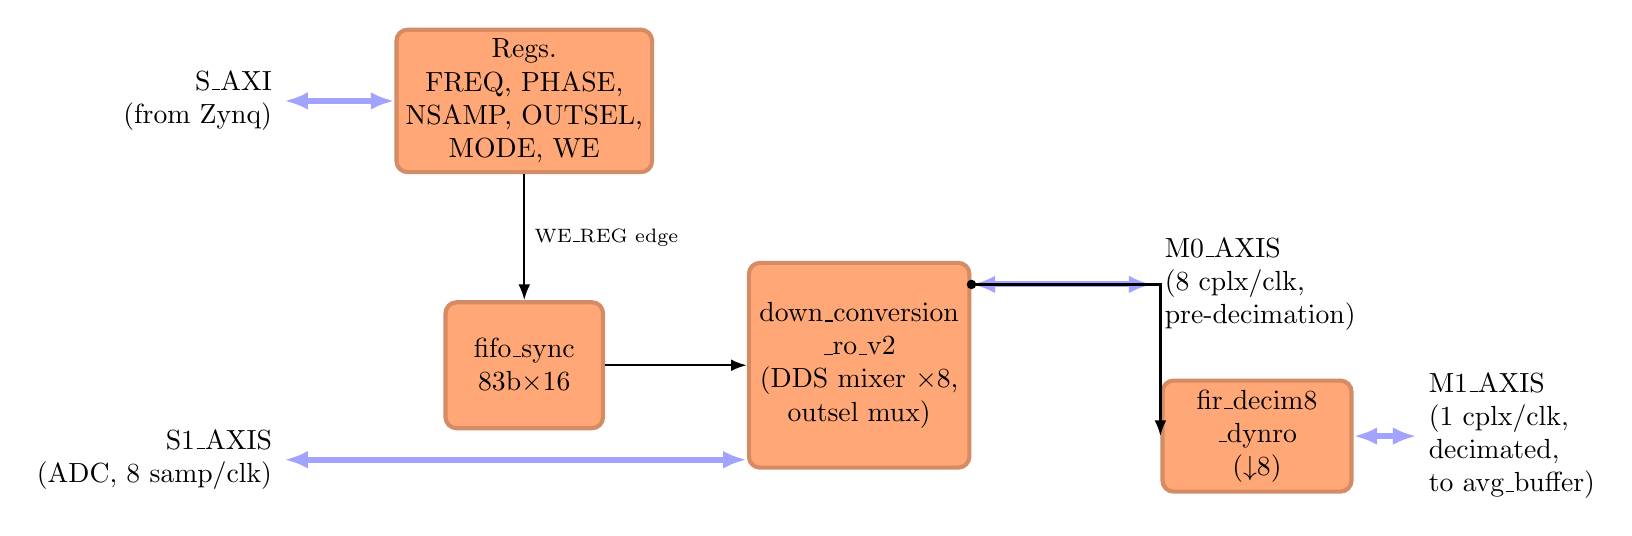
\begin{tikzpicture}
[box/.style={align=center, draw,rounded corners,minimum width=2cm,minimum height=1.2cm,draw={rgb,255:red,213; green,139; blue,99},fill={rgb,255:red,255; green,167; blue,118},line width=1.5pt},
arrow/.style={line width=2.2pt,draw={rgb,255:red,162; green,163; blue,255},{Latex[length=3mm]}-{Latex[length=3mm]}},
single arrow/.style={line width=0.8pt,-{Latex[length=2mm]}},
node distance=0.5cm]

% Registers.
\node[box,minimum height=1.6cm,minimum width=2.6cm] (regs) {Regs.\\FREQ, PHASE,\\NSAMP, OUTSEL,\\MODE, WE};

% Descriptor FIFO.
\node[box,below=1.6cm of regs,minimum height=1.6cm] (fifo) {fifo\_sync\\83b$\times$16};

% Down-conversion (DDS mixer + 3-way outsel mux: product/dds/raw ADC).
\node[box,right=1.8cm of fifo,minimum height=2.6cm,minimum width=2.8cm] (dc) {down\_conversion\\ \_ro\_v2\\(DDS mixer $\times$8,\\ outsel mux)};

% Decimating FIR (reused unchanged from dyn_readout).
\node[box,right=2.4cm of dc,yshift=-0.9cm,minimum width=2.4cm] (fir) {fir\_decim8\\ \_dynro\\($\downarrow$8)};

% s_axi: config registers, from Zynq.
\draw[arrow] ($(regs.west)+(-1.4,0)$) coordinate (s axi in) node[anchor=east,align=right] {S\_AXI\\(from Zynq)} -- (regs.west);

% regs -> fifo (WE_REG rising edge pushes one descriptor).
\draw[single arrow] (regs.south) -- (fifo.north) node[pos=0.5,right,font=\scriptsize] {WE\_REG edge};

% fifo -> down-conversion (freq/phase/nsamp/outsel/mode).
\draw[single arrow] (fifo.east) -- (fifo.east -| dc.west);

% s1_axis: ADC samples in.
\coordinate (temp) at (s axi in |- fifo.west);
\draw[arrow] ($(temp)+(0,-1.2)$) coordinate (s1 in) node[anchor=east,align=right] {S1\_AXIS\\(ADC, 8 samp/clk)} -- (s1 in -| dc.west);

% down-conversion -> m0_axis (pre-decimation output; outsel picks product/dds/raw).
\coordinate (dc out) at ($(dc.north east)+(0,-0.3)$);
\draw[fill] (dc out) circle (1.5pt);
\draw[arrow] (dc out) -- ++(2.3,0) node[anchor=west,align=left] {M0\_AXIS\\(8 cplx/clk,\\ pre-decimation)};

% down-conversion -> fir (same data also feeds the decimating path).
\coordinate (fir in) at (dc out -| fir.west);
\draw[single arrow] (dc out) -- (fir in) -- (fir.west);

% fir -> m1_axis (decimated output).
\draw[arrow] (fir.east) -- ++(0.8,0) node[anchor=west,align=left] {M1\_AXIS\\(1 cplx/clk,\\ decimated,\\ to avg\_buffer)};

\end{tikzpicture}

\end{document}
